\section{Optimal Control of Pitch, Travel and Elevation with and without Feedback}\label{sec:prob4}
In this section, we extend our model to include the remaining states; elevation $e$, and elevation
rate $\dot{e}$. We use a non-linear solver to compute an optimal trajectory in two dimensions,
and additionally constrain the elevation to avoid a restriction shaped as a bell-curve.

\subsection{State-space formulation}
The state-vector is extended with the remaining states,
\begin{equation}
\label{eq:day4_cost}
    x = \begin{bmatrix} \lambda & r & p & \dot{p} & e & \dot{e} \end{bmatrix}^T
\end{equation}
and the elevation setpoint is added to the input-vector
\begin{equation}
    u = \begin{bmatrix} p_c & e_c \end{bmatrix}^T.
\end{equation}
The system is on the usual state-space form (\ref{eq:state_space_axbu}), with
\begin{equation}
    \dot{x} =
    \underbrace{
    \begin{bmatrix}
    0 & 1 &      0     &      0     &      0     &      0    \\
    0 & 0 &    -K_2    &      0     &      0     &      0    \\
    0 & 0 &      0     &      1     &      0     &      0    \\
    0 & 0 & -K_1K_{pp} & -K_1K_{pd} &      0     &      0    \\
    0 & 0 &      0     &      0     &      0     &      1    \\
    0 & 0 &      0     &      0     & -K_3K_{ep} & -K_3K_{ed}
    \end{bmatrix}}_{A_c}
    x +
    \underbrace{
    \begin{bmatrix}
        0       &     0     \\
        0       &     0     \\
        0       &     0     \\
    K_1K_{pp}   &     0     \\
        0       &     0     \\
        0       & K_3K_{ep}
    \end{bmatrix}}_{B_c}
    u
    \label{eq:extended_state_space}
\end{equation}

\subsection{Discretization}
We discretize (\ref{eq:extended_state_space}) using the same method as in section (\ref{sec:prob2}). That is, an approximation of the discrete-time state-space matrices is
\begin{equation}
    A \approx I + hA_c
    \qquad\text{and}\qquad
    B \approx hB_c
\end{equation}
where $I$ is the $6\times6$ identity matrix.

\subsection{Modelling the restriction}
A common reason for using optimal control is to implement restrictions on state or input. This can be used to avoid physical objects or conserve input power. Such restrictions can not be enforced when using only state feedback controllers. In this section, we wish to restrict the helicopter head to move above the bell-shaped curve
\begin{equation}
    e_k \geq \alpha \exp (-\beta (\lambda_k - \lambda_t)^2 )
\end{equation}
for all timesteps $k$ of the horizon. Since this is a non-linear constraint, we can no longer use a linear solver.

\subsection{Objective function}
Since we now have an additional degree of freedom, we extend the cost function (\ref{eq:trajectory_cost}) with an additional term to penalize the usage of elevation
\begin{align}
    \phi &=\sum (\lambda_t - \lambda_f)^2 + r_{p}p_{ct}^2 + r_{e}e_{ct}^2 \\
         &=\sum(x^{T}Qx+u^{T}Ru)
\end{align}
Here, $Q$ and $R$ are diagonal matrices, with unity weight on the travel error, $r_p$ and $r_e$, so that it corresponds with the extended state and input vectors of equation (\ref{eq:day4_cost}). This formulation makes it possible to easily put some weight on the other states as well, if deviation in these states should be penalized.

\subsection{Results open loop}
For controlling the helicopter, we used a horizon of $N=60$ or 15 seconds. We solved the optimization problem using the built-in MATLAB function fmincon, which is an SQP-type solver. This gave an optimal trajectory that looked much the same as in section \ref{sec:prob2} for pitch and travel. In addition, an elevation trajectory just touching the top of the bell curve constraint was also calculated. The suggested horizon of $N=40$ did not terminate in reasonable time, and was therefore replaced by a longer horizon giving reasonable results. The results without feedback were similiar to section (\ref{sec:prob2}), as shown by figure \ref{fig:day4_ol}.

% The real trajectory of travel and elevation tried to follow the optimal solution, but the effects of linearization and having an imperfect model became more and more clear as time passed, and at the end of the horizon, the travel drifted away from the solution just like in section \ref{sec:prob2} since it did not manage to stop correctly.

\begin{figure}[htb]
    \centering
     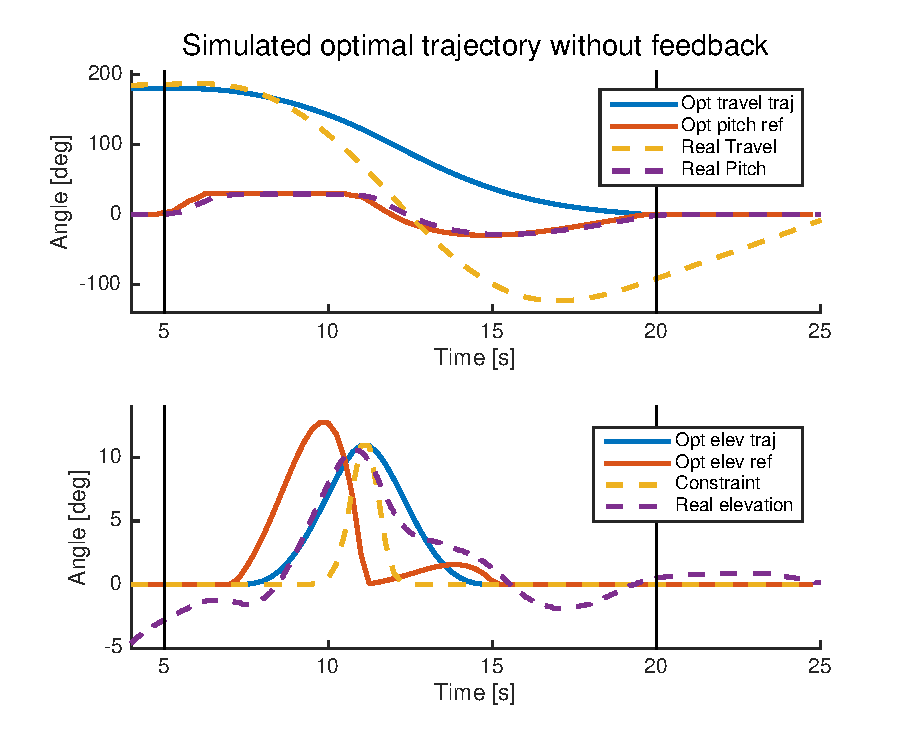
\includegraphics{figures/day4_ol/plot_day4_OL}
    \caption{Problem 4 open loop response}
    \label{fig:day4_ol}
\end{figure}

\subsection{Results closed loop}

Using feedback and LQR, the helicopter managed to follow the calculated trajectory better after some tuning. As in section (\ref{sec:prob3}), it was appropriate to weight deviation in travel (and here elevation as well) more than deviation in pitch. This is again due to modelling and linearization errors, making it preferrable to track the desired travel and elevation trajectories rather than the input sequence. Figure \ref{fig:day4_cl_plot_allQ} compares the travel trajectory for different weights values of $Q_{\text{LQR}}$.

\begin{figure}[ht!]
    \centering
     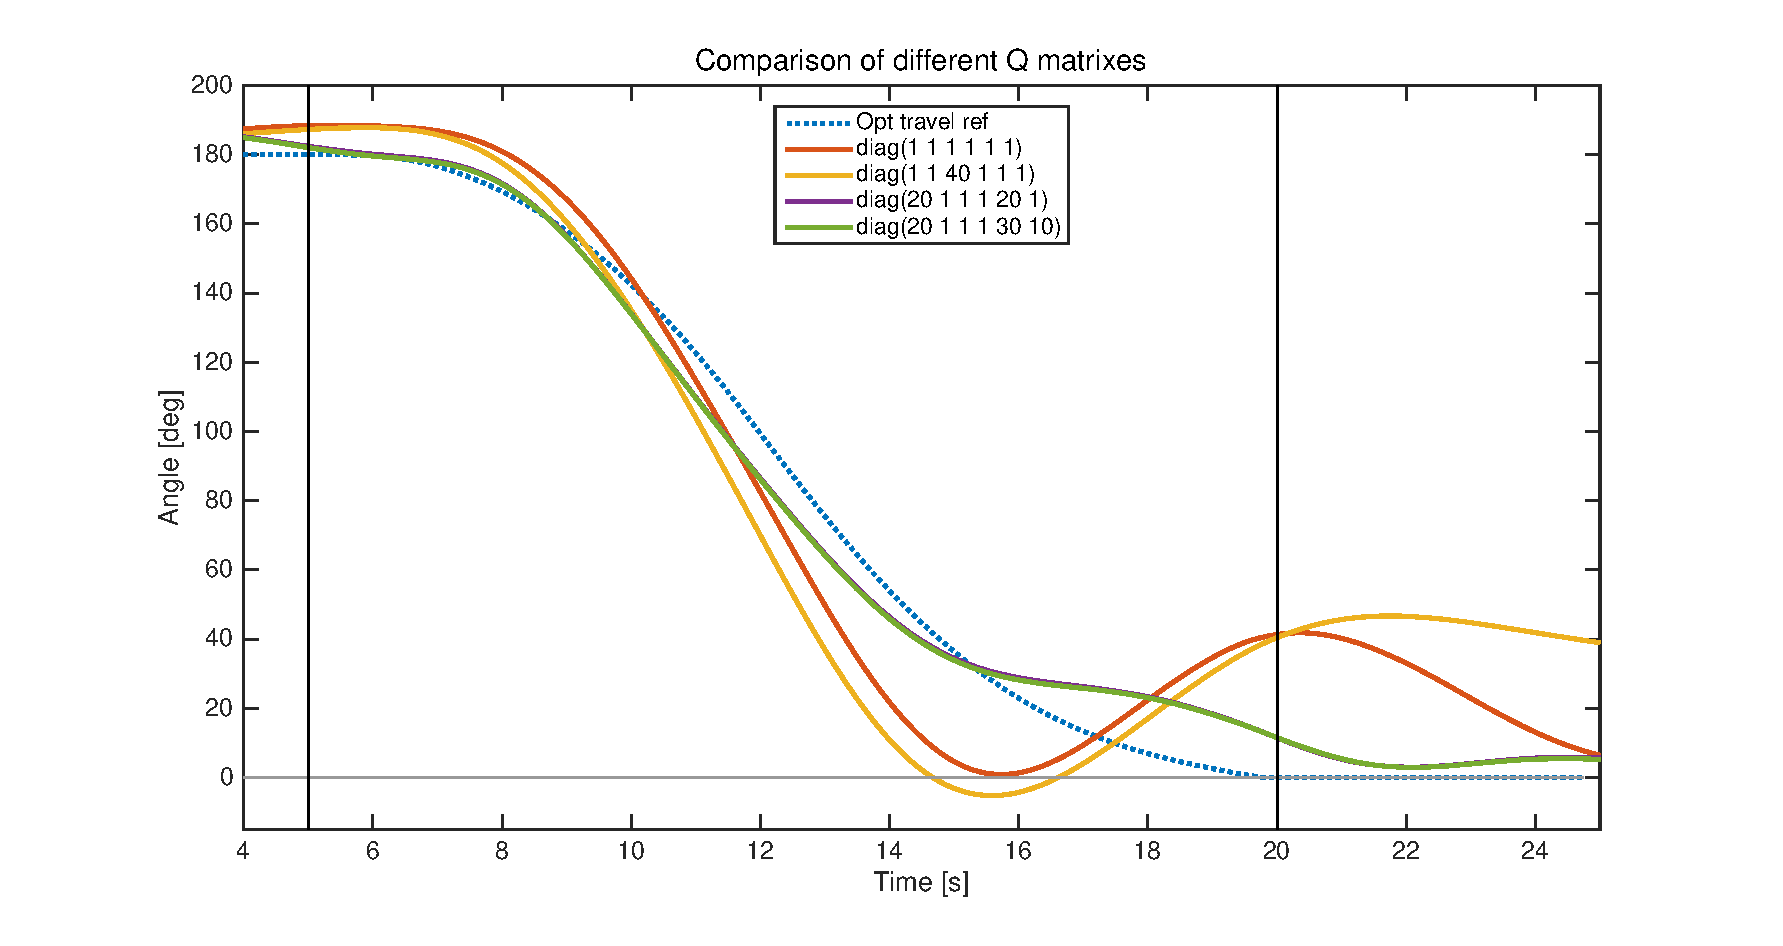
\includegraphics[width=1.0\textwidth]{figures/day4_cl/plot_day4_cl_allQ}
    \caption{Plot day 4 closed loop}
    \label{fig:day4_cl_plot_allQ}
\end{figure}

One thing worth noticing is that the trajectory of elevation consequently fell below the constraint at the peak of the constraint, approximately 11 seconds into the simulation. We believe this is due to the fact that our model suggests that there is no link between the model for elevation, and that of pitch. They are in fact linked, and because of this, the regulator doesn't manage to meet both demands perfectly at the same time, and we get a deviation. If the model would include these crossing terms, the result would probably be better. The problem with this approach is that it leads to a non linear objective function, which takes longer time to compute for the solver.
\begin{figure}[ht!]
    \centering
     \includegraphics[width=0.8\textwidth]{figures/day4_cl/plot_day4_CL_q_20_1_1_1_20_1_marked2}
    \caption{Coupling between pitch and elevation}
    \label{fig:coupling_pitch_elev}
\end{figure}
